\chapter{学写程序} % Introduction chapter suppressed from the table of contents


第四天早上10:00我终于把所有功能写完并通过自动单元测试!\\
(老师说学编码必须动手,但我平时忙于工作,这次趁十一长假做编码练习题。上次做题已经是春节后,在集中隔离期间做过两题。这次的练习题只有十个功能,本来预计可两天完成。)

\begin{longtable}[]{@{}l@{}}
\toprule
\endhead
\begin{minipage}[t]{0.97\columnwidth}\raggedright
练习题 (Problem
Set)------分析美国过去温度变化,提供了美国超过20个城市的每天平均温度。(从1961年到2015年)

\begin{itemize}
\tightlist
\item
  先写基本功能:

  \begin{itemize}
  \tightlist
  \item
    画散点图,回归分析,计算标准差与决定系数 (R\textsuperscript{2} Coef.
    of determination)
  \end{itemize}
\end{itemize}

\begin{itemize}
\tightlist
\item
  分析过去的五六十年数据,来判断美国或全球是否在暖化
\end{itemize}

给学生的文件包:

\begin{enumerate}
\tightlist
\item
  ProblemSet5.pdf : 分成 A、 B 、C、 D、
  E部分,详细说明每部分要开发的功能
\item
  PS5.py 程序模板,学员填入代码
\item
  PS5\_test.py 自动单元测试模块,自动测写好的PS5.py
\end{enumerate}\strut
\end{minipage}\tabularnewline
\bottomrule
\end{longtable}

回顾一下,像我这种Python新手,因为不熟悉Python语言的属性与特性,必须按部就班,一步一步来写,欲速则不达。

更重要是体会到个人如何记录数据并分析:

\begin{longtable}[]{@{}l@{}}
\toprule
\endhead
\begin{minipage}[t]{0.97\columnwidth}\raggedright
\hypertarget{ux8bb0ux5f55ux65f6ux95f4}{%
\subsubsection{记录时间}\label{ux8bb0ux5f55ux65f6ux95f4}}

十多年前我在美国考CMMI培训师,被观察时,
观察老师会在培训后告诉我,每一个模块用了多少时间,与计划对比。
从此以后每次培训我都会习惯记录每个模块所花的时间。

\hypertarget{ux600eux6837ux505a}{%
\subsubsection{怎样做}\label{ux600eux6837ux505a}}

培训时,我都会在桌上放一数字电子钟,记录每一个模块的开始时间与结束时间。上完一天课,晚上在电子表单计划时间旁边写上每个模块的实际时间。
这三天半,我也是用这种方式记录每个模块的时间。

\hypertarget{ux8bb0ux5f55ux7f3aux9677}{%
\subsubsection{记录缺陷}\label{ux8bb0ux5f55ux7f3aux9677}}

因为每个功能都很小,不到20行, 所以没有正式把缺陷与返工工作量记下来。
尤其是一些小的语法错误问题立马就改正了。
但影响较大的重大缺陷,我会记在模块旁边,算是这个模块花的时间。

个人记录实际时间没有想象中这么困难,
只要每天晚上简单按当天本子的数据更新电子表单,避免遗忘。

%\href{文件:PspLogScreenshot_2021-10-06_174917.png}{500px}

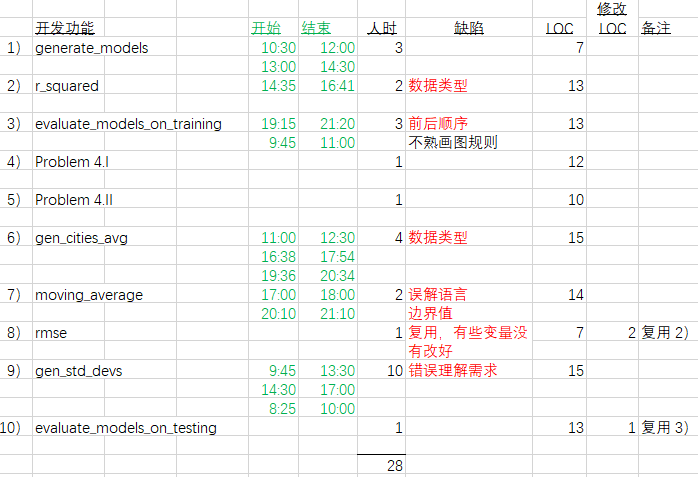
\includegraphics[width=10cm]{PspLogScreenshot20211006174917.png}

\hypertarget{ux56deux987eux5206ux6790}{%
\subsubsection{回顾分析}\label{ux56deux987eux5206ux6790}}

整个编程结束后,写上每一个模块的实际代码行数。注意:如果模块是复用其他模块代码,便需要注明改动的代码行数。例如:evaluate\_models\_on\_testing13行只修改了1行。

分析:除了标准差模块(gen\_std\_devs)以外,其他功能都能在1-3个小时之内完成。

计算标准差的功能花了 10
小时,问题出在我编码时没有详细看需求。开始以为是求每个城市的温度标准差。
然后再求标准差的平均数。\\
测试不通过后,
也没有再看需求便假定求当年几个城市所有当年每天温度的标准差,还是不对。
到了第四天早上再看看 ProblemSet5.pdf
需求描述才知道我一直误解了这功能需求。

\texttt{gen\_std\_devs~~对应每一输入年份,返回一个数值,依据以下计算:}~\\
\texttt{~1)按输入的所有城市,计算当年每一天的平均温度(所有城市的平均)}~\\
\texttt{~2)计算当年每一天平均温度的标准差}~\\

所以如按我本来的算法,算一个城市是正确,但两个或者多个城市的时候,答案就比正确答案大。

针对这个计算标准差问题,一直以为是语法问题公式计算错误问题。
但我用一些简单的数据检验去,未能发现任何不正常。
来来去去都没有实际的进展,差点想放弃。

\hypertarget{ux7ecfux9a8cux6559ux8bad}{%
\subsubsection{经验教训}\label{ux7ecfux9a8cux6559ux8bad}}

每次评审后我都会跟客户说,要做好需求评审,才能降低返工工作量。
这次编码实验的经验告诉我,如果前期过程有缺陷遗漏,
后面确实要付出很大的代价。(10小时是平均2小时(1 -
3小时)的5倍,还只是15行代码的小功能。在实际软件开发项目中,经验丰富的编码员应不像我这么笨,但估计因前面过程遗漏缺陷在系统集成后,测试才发现的返工量应也不止5倍!)

有了数据记录,这类宝贵个人经验便可以转化为改进(不仅仅是一个印象)。例如,可以把这些变成个人风险清单的检查项
-\/-避免同类问题再发生。

\hypertarget{ux7ed3ux8bba}{%
\subsubsection{结论}\label{ux7ed3ux8bba}}

统计工作量与缺陷数据要从个人开始,并在回顾分析各种缺陷类型的返工量,找根因,制定对应措施,下次可以避免同类缺陷,我们才有动力继续收集数据。\strut
\end{minipage}\tabularnewline
\bottomrule
\end{longtable}

\hypertarget{ux5176ux4ed6ux7f16ux7801ux7ecfux9a8cux6559ux8bad}{%
\subsection{其他编码经验教训}\label{ux5176ux4ed6ux7f16ux7801ux7ecfux9a8cux6559ux8bad}}

\begin{itemize}
\tightlist
\item
  最佳实践: 尽量用最小的行数完成功能

  \begin{itemize}
  \tightlist
  \item
    像Python这类成熟的语言,绝大部分的功能都已经具备
  \item
    尽量避免基础方法编写一个已有的功能(reinvent the
    wheel),除了耗费时间外,还会写多错多
  \end{itemize}
\end{itemize}

\begin{itemize}
\tightlist
\item
  写任何程序前必须先有自动化测试用例

  \begin{itemize}
  \tightlist
  \item
    虽然自己可以先想一些数据自己简单测一下
  \item
    但替代不了另外一个人写的测试用例。跑通才有信心程序正确
    (所以自动单元测试是使用最多的程序)
  \end{itemize}
\end{itemize}

\begin{itemize}
\tightlist
\item
  架构与设计很重要

  \begin{itemize}
  \tightlist
  \item
    校方除了提供测试脚本外,还提供了写程序的模板 (PS5.py)
  \item
    每个功能都明确,输入是什么,什么数据类型,输出是什么
  \item
    学员自己只需要填写实现的代码部分
  \end{itemize}
\end{itemize}

\begin{itemize}
\tightlist
\item
  先把握好新功能的用法与结果

  \begin{itemize}
  \tightlist
  \item
    前面发现不少缺陷,是因为不清楚某功能的用法
  \item
    在写代码之前,自己应开个沙盘,用小程序先试验一下这计算功能有什么参数,会出什么结果
  \end{itemize}
\end{itemize}

\begin{itemize}
\tightlist
\item
  先评审后测试

  \begin{itemize}
  \tightlist
  \item
    在跑程序之前,屏幕展示或打印出刚写好的代码,用铅笔在白纸上按程序的逻辑,从头思考一下每个数据的种类和中间的变化
  \item
    盲目地去跑程序或测试,最终只得出测试失败,但还不清楚错在哪里,如何修改。所以不如在跑程序或测试前,自己先动脑筋模拟一次,仔细想通每个数据的变化
  \end{itemize}
\end{itemize}

\hypertarget{ux53cdux9988-1}{%
\section{反馈 1}\label{ux53cdux9988-1}}

\textbf{问}:现在越来越多是敏捷开发和低代码开发,我们现在已经把代码复用作为一个考核机制,而不是把代码效率作为机制了(代码效率已经很难体现),所以单看写编码效率参考意义不大。\\
\textbf{答}: 很同意现代软件开发已经很少从零开始写,很多都复用。
这是应用型平台发展的趋势, 快速响应交付要求也是趋势

对于代码复用,需要考虑的是:
很多缺陷是由于复用代码时没有把参数改正导致,例如有研究发现大型软件如X-window有接近20\%的代码是复制粘贴过来,但也正是这些复制粘贴代码,后面被发现有缺陷(大部分由于复制粘贴没改正变量/参数)。所以虽然是复用代码,还需要记录花了多少工时,有多少缺陷返工。针对这问题,我们也在寻找开发工具来扫描代码中的复制粘贴与可能代码缺陷。我3天半编码过程中,也遇过好几次这类问题。所以在没有可靠的代码扫描工具前,不如把这类问题作为代码评审检查项,尽量在开发评审时发现修正,避免后期的大量返工。

明白以上原则后,我们可以变通地记录所花工作量:例如,规模除了用代码行数,也可以用功能
/ 接口 / 使用组件等单位衡量规模,
并识别那些是复用,把新开发/复用分开。以今次Python编程为例,我总共开发了8个功能(problem
4.I、4.II 不算功能):

%Screenshotfrom20221219222055.png

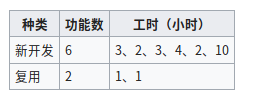
\includegraphics[width=10cm]{Screenshotfrom20221219222055.png}

如不考虑花费了10工时那功能,其他5个花了2、2、3、3、4工时,马上得出
Q1(P25)=2、Q2(P50)=3、Q3(P75)=3 小时,复用是 1
小时,按这种功能数得出来的基线可能比用代码行数来算更好用。

效率考虑的是工作量,也就是成本,是项目目标项,但复用度不是目标项。
衡量复用可以帮助分析效率与复用的关系,成本与复用的关系,但复用不应该作为考核项。
复用的目的,应该是降低成本、工作量等,不是为了质量,复用不一定导致质量的改善。

\hypertarget{ux53cdux9988-2}{%
\section{反馈 2}\label{ux53cdux9988-2}}

客户:你写的分享文章都很好,但不知道如何能解决我们实际遇到的问题。\\
我:有什么问题?\\
客户:问题很多,例如你们前面教的功能点方法,大部分的项目经理/产品经理都没真正用上,很多开发人员天天忙于救火,缺乏总体产品设计;因为开发出来的问题多,现场实施人员就无法解决客户现场的问题,最终还是要开发人员出手解决。\\
我:你们的组长如何分配工作给编码人员开发?\\
客户:很多时候,因为时间紧张,只是简单说要开发什么,如果赶工组长甚至会自己动手直接把代码改好。\\
我:这3天半的编码经验提醒我架构与单元测试都非常重要,如果老师没有在练习题把每个模块的输入输出和要通过的单元测试预先写好,随便让学生编码的话,我估计大部分学生都无法完成。所以组长不应该自己写代码,而是设计好整个架构有那些模块与每个的输入输出。你们都学过功能点方法,
以功能点为基础的数据分析,纵向可以展现个人进步,横向可以衡量个人之间的工作效率差异,
你们开发人员需要填工时么?\\
客户:要的,但是否正确,难以判断。\\
我:你们开发人员有评级制度吗?\\
客户:去年开始,但主要依赖主管打分。\\
我:如果你们要求把个人统计分析数据反映的工作效率差异及实际改进作为升级的必须条件,他们才有动力来统计个人的工作量,好比你打算半年后参加马拉松半马,你才有动力定计划,并记录每天的速度。如果每个开发人员都有用本子记录每天的开发时间,团队就可以在每2周回顾时整个团队一起利用迭代数据分析本迭代的缺陷主要源自那个过程(需求,设计,编码等)。然后再针对主因制定下个迭代的改进措施。\\
客户:理解了,你希望他们可以自己从数据发现自己的问题并改善。\\
我:你说的很对,不能单靠你们2位公司PMO分析数据,要求他们做改进,因为他们很可能不认同你们的分析结果。\\
从以上的客户对话,可以了解到要量化管理软件开发必须从个人开始,因为团队的能力是建基于个人能力之上。投入和产出成正比,在量化记录上投入少量时间,得到的是项目个人和团队的进步和成倍产出。\\

\hypertarget{references}{%
\section{References}\label{references}}

1. MIT OCW 6.0002 Fall 2016 Introduction to Computational Thinking and
Data Science - Problem Set 5\\




